\chapter{Linear programming for approximation algorithms}

\textbf{\textsc{Content note}}: \emph{Part of this chapter is taken from \href{https://github.com/Halolegend94/uni_social_behavioral_networks/blob/master/chapters/ch05-densest-subgraph.tex}{this repo} by \href{https://github.com/Halolegend94}{Cristian Di Pietrantonio}.}
\vspace{2ex}

In this chapter Linear Programming is introduced as a tool to build approximation algorithms. In particular, we use the \textit{Densest Subgraph} problem (DSG for short) as a practical example, because some practitioners believe that it is a good primitive to find community of people; also, this problem is in $P$ and we will solve it through linear programming.

You can read more about this \href{https://github.com/Halolegend94/uni_social_behavioral_networks/blob/master/main.pdf}{here}.

\section{Linear Programming}

Linear programming, or \lp{} in short, is a method to achieve the best outcome, such as maximum profit or lowest cost, in a mathematical model whose requirements are represented by linear relationships. It is arguably the most important technique when it comes to approximation algorithms, and many heuristics built with other methods can be mapped to a corresponding \lp{} instance.

More formally, linear programming is a technique for the optimization of a linear \emph{objective function}, subject to linear equality and linear inequality \emph{constraints}. Its feasible region is a convex polytope, which is a set defined as the intersection of finitely many half spaces, each of which is defined by a linear inequality. Its objective function is a real-valued affine (linear) function defined on this polyhedron. A linear programming algorithm finds a point in the polytope where this function has the smallest (or largest) value if such a point exists.

\begin{definition}[Primal linear program]\label{def:lpprimal}
    A \emph{primal} linear program has the specific purpose to maximize its objective function:
    \begin{equation*}
        \max(c_1 x_1 + c_2 x_2 + \ldots + c_n x_n)
    \end{equation*}

    where all of the variables are real and nonnegative; the constraints are of this form;
    \begin{equation*}
        \begin{cases}
            a_{1 1} x_1 + a_{1 2} x_2 + \ldots + a_{1 n} x_n &\leq b_1 \\
            a_{2 1} x_1 + a_{2 2} x_2 + \ldots + a_{2 n} x_n &\leq b_2 \\
            \quad \vdots                                     &         \\
            a_{m 1} x_1 + a_{m 2} x_2 + \ldots + a_{m n} x_n &\leq b_m \\
        \end{cases}
    \end{equation*}
\end{definition}

Note that, if there were no constraints, the optimization problem would have been trivial.

Furthermore, the assumption of nonnegative $x_i$ is made without loss of generality; to model a negative variable, it suffices to obtain it from other positive variables such as $y = x_1 - x_2$.

A primal \textsc{lp} can also be written more compactly in matrix form:
\begin{equation}\label{primal-matrix}
    \begin{aligned}
        &\max(\overline{c}^T \overline{x}) \\
        &A \overline{x} \leq \overline{b} \\
        &\overline{x} \geq \overline{0}
    \end{aligned}
\end{equation}


where:

\[
    \overline{x} =
    \begin{pmatrix}
        x_1 \\ x_2 \\ \ \vdots \\ x_n
    \end{pmatrix}
    \quad
    A =
    \begin{pmatrix}
        a_{11} & a_{12} & \cdots & a_{1n} \\
        a_{21} & a_{22} & \cdots & a_{2n} \\
        \ \vdots & \ \vdots &  & \ \vdots \\
        a_{n1} & a_{n2} & \cdots & a_{mn}
    \end{pmatrix}
    \quad
    \overline{b} =
    \begin{pmatrix}
        b_1 \\ b_2 \\ \ \vdots \\ b_m
    \end{pmatrix}
    \quad
    \overline{c} =
    \begin{pmatrix}
        c_1 \\ c_2 \\ \ \vdots \\ b_n
    \end{pmatrix}
\]

\begin{definition}(Dual linear program)\label{def:lpdual}
    A \emph{dual} linear program, unlike a primal one, aims to minimize its objective function; its matrix form is:
    \begin{equation}\label{dual-matrix}
        \begin{aligned}
            &\min(\overline{y}^T \overline{b}) \\
            &\overline{y}^T A \geq \overline{c} \\
            &\overline{y} \geq \overline{0}
        \end{aligned}
    \end{equation}
    
    Note that it uses the same (transposed) coefficient and constant matrices of a primal, but the variable vector has dimension $m$ instead of $n$. This means that changing $\max$ into $\min$ and letting any constraint become a variable and viceversa is required to pass from the primal to the dual.
\end{definition}

\begin{theorem}[Weak Duality]\label{thm:weak-duality}
    If $\overline{x}$ is a feasible solution to the primal and $\overline{y}$ is a feasible solution to the dual, then
    \begin{equation}
        \overline{c}^T \overline{x} \leq \overline{y}^T \overline{b}
    \end{equation}
\end{theorem}

\begin{proof}
    \[
        \overline{c}^T \overline{x} \leq (\overline{y}^T A)\overline{x} = \overline{y}^T (A \overline{x}) \leq \overline{y}^T \overline{b}
    \]
    where the first inequality holds by definition of dual, and the second by definition of primal.
\end{proof}

Given a primal \lp{}, the usual way to solve it is to guess a solution $\overline{x}$, check that it satisfies the constraints, and then evaluate how good it is by using the objective function. To know if the solution is sufficienlty close to optimal, the same process can be applied on the corresponding dual \lp{} with another solution $\overline{y}$. If the costs of both guesses are close, then the chosen solutions are indeed close to optimal.

\begin{theorem}[Strong Duality]\label{thm:strong-duality}
    If $\overline{x}$ is an optimal solution to the primal and $\overline{y}$ is an optimal solution to the dual, and if $\overline{c}^T \overline{x}$ and $\overline{y} \overline{b}$ are finite, then the solutions are the same:
    \begin{equation}
        \overline{c}^T \overline{x} = \overline{y} \overline{b}
    \end{equation}
\end{theorem}

In essence, when the solutions for a primal and its corresponding dual tend to equate each other, then they are the optimal solution.

It is a common approach to transform a given combinatorial problem into a linear one, then solve the latter, which is proven to require polynomial time,\footnote{This is true because the variables are real. Linear programming with integers is known to be an \textsc{np}-complete problem} and then transform the solution to the linear problem in a solution to the original.


\section{Densest subgraph}\label{sec:densest-subgraph}

\subsection{A linear program to solve the densest subgraph problem} \label{sec:dsp-lp}

We are interested in this problem since it allows to find communities into social networks.

\begin{definition}[Induced subgraph]
    Given a graph $G(V, E)$ and a subset of its vertices $S$, the induced graph on $S$, denoted as $G[S]$, is the subgraph $H(S, \powerset_2(S) \cap E(G))$.
\end{definition}

\begin{definition}[Densest subgraph]\label{densest-subgraph}
    The densest subgraph of $G(V, E)$ is an induced subgraph $G[S]$ on some subset $S$ with the largest average degree; in other words, $S$ is such that the density of the graph $f(S) = \frac{|E(S)|}{|S|}$ is maximized.
\end{definition}

Note that, by maximizing the density of a subgraph, its average degree $\frac{2 \abs{E(S)}}{\abs{S}}$ is also maximized. This is a particular approximation problem, since it can actually be solved exactly in polynomial time.

\begin{figure}[ht]
    \centering
    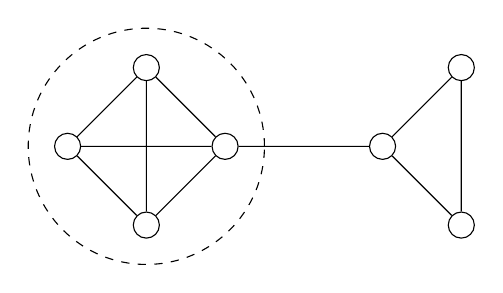
\begin{tikzpicture}[node distance = 20mm]
        \draw
            (0, 1)  node (a) [draw, circle] {}
            (0, -1) node (b) [draw, circle] {}
            (-1, 0) node (c) [draw, circle] {}
            (1, 0)  node (d) [draw, circle] {}
            (3, 0)  node (e) [draw, circle] {}
            (4, 1)  node (f) [draw, circle] {}
            (4, -1) node (g) [draw, circle] {}
            
            (a) -- (b)
            (a) -- (c)
            (a) -- (d)
            (b) -- (c)
            (b) -- (d)
            (c) -- (d)
            (d) -- (e)
            (e) -- (f)
            (e) -- (g)
            (f) -- (g);

            \draw[dashed] (0, 0) circle (1.5);
    \end{tikzpicture}
    \caption{An example of densest subgraph $G[S]$}
    \label{fig:densest-subgraph}
\end{figure}

Here is a primal \lp{} model of this problem:
\begin{equation}
    \begin{aligned}\label{lp-densest-subgraph}
    &\max \left( \sum_{\{i, j\} \in E(G)}X_{\{i, j\}} \right) \\
    &\begin{cases}
        X_{\{i, j\}} \leq Y_i   & \forall \{i, j\} \in E(G) \\
        X_{\{i, j\}} \leq Y_j   & \forall \{i, j\} \in E(G) \\
        \sum_{i=1}^n Y_i \leq 1 & \forall i \in V(G) \\
    \end{cases} \\
    &X_{\{i, j\}}, Y_i \geq 0  \qquad \forall \{i, j\} \in E(G) \quad \forall i \in V(G)
    \end{aligned}
\end{equation}

\todo{The lesson has been essentially structured around Charikar's paper ``Greedy approximation algorithms for finding dense components in a graph'' which, in one author's opinion, fails to relate at first glance this linear program to the problem. There is a more accessible thesis \href{https://gupea.ub.gu.se/bitstream/2077/49476/1/gupea_2077_49476_1.pdf}{here}, which starts from a linear program that is arguably more relatable to the original problem, and proceeds to convert it to this form, with the added bonus of showcasing how to linearize nonlinear objective functions and constraints. Might decide to replicate it here.

However, the lemmata and proofs that follow are found only in Charikar's article}

Starting from the objective function, we want something that says ``get as many edges as possible in the final graph''; so, it seems natural to maximize the number of edges we can put in the final subset of nodes. Observe, though, that we cannot maximize $f(S)$ since it is not linear. One can take another approach and look only at the numerator. We define a variable $X_{\{i, j\}}$ to be the fractional amount of edge $\{i, j\}$ that is put inside the solution. The objective function is
\begin{equation}
    \max \left( \sum_{\{i, j\} \in E(G)}X_{\{i, j\}} \right)
\end{equation}

For each edge, we cannot pick that edge fractionally more than the amount with which we pick one of its endpoints. For example, if we pick $\{i, j\}$ for $\frac{1}{2}$ of its entirety, then it is the case that we had to pick both $i$ and $j$ for at least $\frac{1}{2}$. This can be expressed introducing a variable $Y_i$ for each node $i$, representing the fractional amount with which we pick node $i$; then, we can say that
\begin{equation}\label{eq:dsp_x_constraints}
    \begin{aligned}
        X_{\{i, j\}} &\leq Y_i \\
        X_{\{i, j\}} &\leq Y_j
    \end{aligned}
\end{equation}


Up until now the LP is unbounded. We now need to model the denominator by saying that the total amount with which nodes of the graph are picked must be limited; we can think of that amount being, say, 1 to normalize it. Making the denominator a constant allows us to linearize the objective function.
\begin{equation}\label{eq:dsp_y_constraint}
    \sum_{i = 1}^n Y_i \leq 1.
\end{equation}

Finally, the variables must be non-negative:
\begin{equation}
    X_{\{i, j\}}, Y_j \geq 0
\end{equation}

The goal is to prove that the optimal solution $OPT_{LP}$ of this \lp{} is equal to the optimal solution of the original densest subgraph problem $f(S^*)$, where $S^*$ is the densest subgraph of $G$. To do so we need the following steps:
\begin{enumerate}
    \item There exists a feasible solution to the \lp{} having value $f(S)$;
    \item $OPT_{LP} \geq f(S^*)$;
    \item $f(S^*) \geq OPT_{LP}$.
\end{enumerate}

\begin{lemma}\label{lem:dsp-feasibility}
    Given a graph $G(V, E)$, for any nontrivial subset $S$ of $V$, there exists a feasible solution to the \lp{} stated above, having value $f(S) = \frac{|E(G[S])|}{|S|}$, which is the subgraph's density.
\end{lemma}

\begin{proof}
    Define:
    \[
        Y_i := \begin{cases}
            \frac{1}{|S|}   & \textsc{if } i \in S \\
            0               & \textsc{else}
        \end{cases}
    \]
    
    Remember that the variables $Y_i$ represent how much of each node in the graph we are taking, this definition states that we split the unit among the nodes in the set $S$. Then let:
    
    \[
        X_{\{i, j\}} = \begin{cases}
            \frac{1}{|S|}   & \textsc{if } \{i, j\} \in E(G[S]) \\
            0               & \textsc{else}
        \end{cases}
    \]
    
    For this solution to be feasible, all constraints are checked. Starting with inequality \ref{eq:dsp_y_constraint}, notice that if a variable $Y_i$ models a vertex not in $S$, then it does not contribute to the sum in the constraint; conversely, if such vertex is in $S$, then it evaluates to the same constant value:
    \[
        \sum_{i \in V(G)} Y_i = \sum_{i \in S} Y_i = \sum_{i \in S} \frac{1}{|S|} = |S| \frac{1}{|S|} = 1
    \]
    
    Then proceed with the inequalities of type \ref{eq:dsp_x_constraints}. Let $\{i, j\} \in E(G)$; again, there are two cases:
    \begin{itemize}
        \item $\{i, j\} \not\in E(G[S])$: In this case, $X_{\{i, j\}} = 0$ by definition, and the constraints are trivially satisfied;
        
        \item $\{i, j\} \in E(G[S])$: This implies that $\frac{1}{|S|} \leq Y_i, Y_j$. Since the edge is assumed to be in the subgraph, then its endpoints must be in $S$, which entails that $Y_i, Y_j = \frac{1}{|S|}$, satisfying the constraints.
    \end{itemize}
    
    The solution is proven to be feasible. Evaluating the objective function:
    \[
        \sum_{\{i, j\} \in E(G)} X_{\{i, j\}} = \sum_{\{i, j\} \in E(G[S])} X_{\{i, j\}} = \sum_{\{i, j\} \in E(G[S])} \frac{1}{|S|} = \frac{\abs{E(G[S])}}{|S|} = f(S)
    \]
\end{proof}

\begin{corollary}
    Let $OPT_{\lp}$ be the value of the optimal feasible solution to the \lp{} obtained from some subset $S \subseteq V$, and let $S^*$ be the densest subgraph of $G$, then:
    \[
        f(S) = OPT_{LP} \geq OPT = f(S^*) = \frac{\abs{E(S^*)}}{\abs{S^*}}.
    \]
\end{corollary}

In other words, the consequence of constructing the solution used to prove \ref{lem:dsp-feasibility} is that the \lp{}'s optimal value is never worse than the original densest subgraph problem's optimal value.

\begin{lemma}\label{l:dsp-geq-lp}
    Let $\{X_{\{i, j\}}, Y_i\}$ be an optimal solution to the linear program in \ref{lp-densest-subgraph}, having value $v$. Then $\exists S \subseteq V : f(S) \geq v$.
\end{lemma}

\begin{proof}
    To prove this lemma, we will proceed step by step claiming some properties that will help us to reach our goal.
    
    \begin{claim}\label{cl:dsp-1}
        For an optimal solution, the following property holds:
        \[
            \forall \{i, j\} \in E(G) \quad X_{\{i, j\}} = \min(Y_i, Y_j)
        \]
    \end{claim}
    \begin{proof}
        Assume that this was not the case: $\exists\ X_{\{i, j\}} < \min(Y_i, Y_j)$. Then the value of $X_{\{i, j\}}$ can be increased up to $\min(Y_i, Y_j)$, which in turn increases the objective function's value while keeping the solution feasible. It entails that $X_{\{i, j\}}$ wasn't the optimal value, which is a contradiction.
    \end{proof}

    Let $\{X_i, Y_i\}$ be an optimal solution, fix a parameter $r$ and let:
    \begin{align}
        S(r) &:= \{ i \in V(G) : Y_i \geq r\}                   & \label{dsp-sr} \\
        H(r) &:= \{ \{i, j\} \in E(G) : X_{\{i, j\}} \geq r\}   & \label{dsp-er}
    \end{align}

    We are defining two parametric sets: $S(r)$ contains all the vertices $i$ such that $Y_i \geq r$, and as $r$ increases, it increasingly shrinks. $H(r)$ is the edges' analogue.
    
    \begin{claim}\label{cl:dsp-2}
        For any value of $r$ between $0$ and $\max_i(Y_i)$, the edges in $H(r)$ will be exactly the ones induced on $S(r)$:
        \[
            \forall\ 0 \leq r \leq \max_i(Y_i) \qquad \{i, j\} \in H(r) \iff (i, j \in S(r) \wedge \{i, j\} \in E(G))
        \]
        Or alternatively:
        \[
            \forall\ 0 \leq r \leq \max_i(Y_i) \qquad H(r) = E(G[S(r)])
        \]
    \end{claim}

    \begin{proof}
        \begin{align*}
                       \{i, j\} \in H(r) 
            \iff&\     X_{\{i, j\}} \geq r          & \tag{by [\ref{dsp-er}]} \\
            \iff&\     \min(Y_i, Y_j) \geq r        & \tag{by claim [\ref{cl:dsp-1}]} \\
            \iff&\     Y_i \geq r \wedge Y_j \geq r & \\
            \implies&\ i, j \in S(r)                & \tag{by [\ref{dsp-sr}]}
        \end{align*}

        Knowing that $\{i, j\} \in H(r)$ also implies that $\{i, j\} \in E(G)$ completes the proof.
    \end{proof}

    The next steps require to deal with the continuous nature of $r$, for both of the parameterized subsets $S(r)$ and $H(r)$. Focusing on $S(r)$, let $\pi$ be a total ordering over the variables $Y_i$ in the solution, such that their values are sorted in increasing order, and define an additional variable $Y_0$ to be the constant 0:
    \[
        0 = Y_{\pi(0)} \leq Y_{\pi(1)} \leq Y_{\pi(2)} \leq \dots \leq Y_{\pi(|V|)} = \max_i(Y_i)
    \]

    % Captions do not like \abs
    \begin{figure}[ht]
        \centering
        \includegraphics[scale = 0.4]{dsp-integral}
        \caption{A representation of the integral $\int_0^{\max_i(Y_i)} |S(r)| dr$.}
        \label{fig:dsp-integral}
    \end{figure}

    In the perspective of such ordering, $S(r)$ can be plotted in a function graph on the real axis of $r$ where the values of $Y_i$ lie; such function graph is shown in figure \ref{fig:dsp-integral}. With some careful observations, it is possible to transition from a continuous interpretation of the area underlying the function to a discrete one:

    \todo{Figure \ref{fig:dsp-integral} fails to convey a clear, most general case of this perspective, many improvements can be made}
    
    \begin{claim}\label{cl:dsp-3}
        \[
            \int_0^{\max_i(Y_i)} \abs{S(r)} dr = \sum_{i = 1}^n Y_i
        \]
    \end{claim}

    \begin{proof}
        The area underlying the function $|S(r)|$ can be exactly partitioned into $n$ rectangles, where each one is the integral computed between two variables $Y_{\pi(i - 1)}$ and $Y_{\pi(i)}$. The width of such a rectangle will be $Y_{\pi(i)} - Y_{\pi(i - 1)}$, whereas the height shall be $n - i + 1$ as a consequence of the ordering on $Y_i$ enforced by $\pi$. Therefore:
        
        \begin{align*}
               \int_0^{\max_i(Y_i)} \abs{S(r)} dr
            &= \sum_{i = 1}^n (Y_{\pi(i)} - Y_{\pi(i - 1)}) (n - i + 1)                             & \text{(by geom. interpretation of integral)} \\
            &= \sum_{i = 1}^n Y_{\pi(i)} (n - i + 1) - \sum_{i = 1}^n Y_{\pi(i - 1)} (n - i + 1)    & \\
            &= \sum_{i = 1}^n Y_{\pi(i)} (n - i + 1) - \sum_{i = 0}^{n - 1} Y_{\pi(i)} (n - i)      & \text{(by index shift)} \\
            &= \sum_{i = 1}^n Y_{\pi(i)} (n - i + 1) - \sum_{i = 1}^n Y_{\pi(i)} (n - i)            & \left( \begin{aligned} i = 0 &\implies Y_0 = 0 \\ i = n &\implies (n - n) = 0 \end{aligned} \right) \\
            &= \sum_{i = 1}^n Y_{\pi(i)} = \sum_{i = 1}^n Y_i                                       & \text{(order does not matter)}
        \end{align*}
        
    \end{proof}
    
    \begin{claim}\label{cl:dsp-4}
        \begin{equation}
            \int_0^{\max_i(Y_i)} |H(r)|dr = \sum_{\{i, j\} \in E(G)} X_{\{i, j\}}.
        \end{equation}
    \end{claim}

    \begin{proof}
        Proven analogously as for claim \ref{cl:dsp-3}.
    \end{proof}
    
    \begin{claim}\label{cl:dsp-5}
        There exists a value $r \in [0, \max_i(Y_i)]$ such that $\abs{H(r)} \geq v \abs{S(r)}$. This entails that, for such value $r$, there is a solution value that is at least the optimum $v$:
        \[
            f(S(r)) = \frac{|H(r)|}{|S(r)|} \geq v = \sum_{\{i,j\} \in E(G)} X_{\{i, j\}}
        \]
    \end{claim}
    
    \begin{proof}
        Assume that, for any valid $r$, it holds that $|H(r)| < v|S(r)|$. Then:
        \begin{align*}
            \int_0^{\max_i(Y_i)} |H(r)| dr          <&\ v \int_0^{\max_i(Y_i)} |S(r)| dr    & \\
            \sum_{\{i, j\} \in E(G)} X_{\{i, j\}}   <&\ v \sum_{i = 1}^n Y_i                & \text{(by claims [\ref{cl:dsp-3}] and [\ref{cl:dsp-4}])} \\
            v                                       <&\ v \cdot 1                           & \text{(by optimality of $\{X_{\{i, j\}}, Y_i\}$)}
        \end{align*}

        which is a contradiction.
    \end{proof}
    \todo{This isn't finished correctly yet}
    At this point we have proved that the LP we gave finds the exact optimal solution for the Densest Subgraph problem.
\end{proof}

\todo{Not sure on how to explain this}
This \lp{} is proven to work as a good model for the Densest Subgraph problem. However, this begets a different question: is there an efficient method for finding the set $S$ using the program's optimal value $v$? Or to put it in another way, how many candidate sets $S$ can there be? In principle infinitely many, but the only ones that matter are given by $r \in \{Y_i : 1 \leq i \leq n\}$ (because of how $S(r)$ is defined). So we try all the $n$ possible values of $r$ and pick the best one.

Note that solving this \lp{} requires polynomial time; however if the graph of interest is a very large one, such as a social graph woth more than 10\ 000 nodes, this method becomes quite intractable. In such scenarios, linear and sublinear approximations are sought for.


\subsection{A greedy algorithm to solve the densest subgraph problem}\label{sec:dsp-greedy}

Here, a greedy algorithm to approximate the optimal solution in linear time is presented. Recall that $f(S)$ is the function defined in [\ref{densest-subgraph}].

\begin{lstlisting}[caption = {The Greedy algorithm to solve the densest subgraph problem}, label = {lst:dsp-greedy}]
algorithm $Greedy(G(V,E))$:
    $S_0 \gets V$
    for $i=1, \ldots, n-1$:
        let $v_{i-1} \in S$ be a node of minimum degree in $G[S_{i-1}]$
        $S_i \gets S_{i-1} - \{v_{i-1}\}$
    return the ``best'' $S_i$ (in terms of its value $f(S_i)$)
\end{lstlisting}

\begin{obs}
    This algorithm runs in $O(|V| + |E|)$ time, i.e., in linear time.
\end{obs}

\begin{thm}\label{thm:dsp-greedy}
    The solution returned by Algorithm [\ref{lst:dsp-greedy}] is a 2-approximation of the optimal solution.
\end{thm}

\begin{obs}
    We will see that Greedy can be analyzed as an implicit LP. We introduce here a picture that will be more clear later, but is useful since now to show that the optimal and the greedy solution are sandwiched between the solutions of the dual and the primal problems underlying this algorithm: see figure [\ref{fig:dsp-plot}].
    \begin{figure}[h!]
        \centering
        \includegraphics[scale=0.4]{dsp-plot}
        \caption{A plot of the optimal and the greedy solution sandwiched between the dual's and the primal's.}
        \label{fig:dsp-plot}
    \end{figure}
\end{obs}

\begin{proof}
    As it often happens in primal-dual proofs, even in this case it will be useful to refer to an underlying algebraic structure, for this proof it will be the \textit{orientation}.
    
    \begin{defn}[Orientation]
        An orientation $\varphi$ of the simple undirected graph $G(V,E)$ is an assignmento f each edge in $E$ to one of its endpoints.
    \end{defn}
    
    \obs There are $2^{\abs{E}}$ possible orientations $\varphi$.
    
    Let's introduce some other definitions that will be useful in the following proof.
    
    \begin{defn}[$\varphi$-degree]
        Given $\varphi$ and $v \in V$, let $d_\varphi(v) = \abs{\{ e : v \in e,\ e \text{ oriented towards } v \text{ by } \varphi \}}$.
    \end{defn}
    
    \begin{defn}[Maximum $\varphi$-degree]
        Given $\varphi$ and $v \in V$, let $\Delta_\varphi = \max_{v \in V}\{d_\varphi(v)\}$.
    \end{defn}

    \pagebreak
    
    What we want to do now is to bound the quality of the optimal solution in terms of some property of all orientations of the graph $G$. The reason is that the algorithm will be analyzed by making it implicitly select an orientation during its execution. Since we are about to show we can bound the value of the optimal solution to DSG by some function of any orientation, this will allow us to give a bound on the quality of the algorithm.
    
    \begin{lem}\label{l:dsp-greedy-1}
        \begin{equation}
            \forall\ \varphi \max_{\emptyset \subset S \subseteq V}\{f(S)\} \leq \Delta_\varphi.
        \end{equation}
    \end{lem}
    
    \begin{proof}
        \begin{flalign*}
            |E(S)| &\leq \sum_{v \in S} d_\varphi(v)&\tag{$*$}\\
            &\leq \sum_{v \in S} \Delta_\varphi(v)&\tag{we upperbound each $d_\varphi(v)$ with $\Delta_\varphi(v)$}\\
            &= |S| \cdot \Delta_\varphi(v)&\\
            &\Downarrow&\tag{by dividing by $|S|$}\\
            \frac{|E(S)|}{|S|}&\leq \Delta_\varphi&
        \end{flalign*}
        The reason of the step marked by $*$ is the following: Pick $e = \{v, w\} \in E(S)$, the orientation $\varphi$ will orient the edge $e$ towards $v$ or $w$, that is, towards some node of $S$, and therefore it will be counted in the sum; Moreover, if we sum up the $\varphi$-degrees, we will be also counting edges that come from nodes outside $S$ to nodes in $S$.
        
        The fact that $f(S) = \frac{|E(S)|}{|S|}$ concludes the proof.
    \end{proof}

    This prove the upper bound part of Theorem [\ref{thm:dsp-greedy}], that is valid $\forall\ \varphi$; now we want to find a lower bound that is close to the optimal solution of the dual LP underlying Greedy [\ref{lst:dsp-greedy}] ($b$ in figure [\ref{fig:dsp-plot}]), and that holds for Greedy as well as for the optimal solution given by the LP [\ref{lp-densest-subgraph}].
    
    This bound will be valid only for the $\varphi$ implicitly built by Greedy, that we will call $\varphi_G$, defined as follows:
    \begin{itemize}
        \item The orientation is created as the algorithm progresses;
        \item At the beginning no edge is directed towards anything;
        \item When Greedy remove a node $w_i$, all the edges incident in $w_i$ and that are still in the graph will be oriented towards $w_i$.
    \end{itemize}
    An example of $\varphi_G$ is given in figure [\ref{fig:dsp-phi}].
    
    \begin{figure}[h!]
        \centering
        \includegraphics[scale=0.4]{dsp-phi}
        \caption{Example of computation of $\varphi_G$}
        \label{fig:dsp-phi}
    \end{figure}

    Note that the algorithm doesn't care about orientations, but we will use this concept in the proof.
    
    \begin{lem}\label{l:dsp-greedy-2}
        Let $M$ be the solution returned by Greedy, i.e., $M := \max_{i = 0, \ldots, n-1}\{f(S_i)\}$, then the following inequality holds:
        \begin{equation}
            \Delta_{\varphi_G} \leq 2M
        \end{equation}
    \end{lem}
    \begin{proof}
        Pick any $S_i$, let $v_i$ be a node of minimum degree in $G[S_i]$:
        \begin{flalign*}
            d_\varphi(v_i) &= \deg_{S_i}(v_i)&\tag{if I remove $v_i$, then $d\varphi(v_i) = d_{S_i}(v_i)$}\\
            &= \min_{v \in S_i}\deg_{S_i}(v)&\\
            &\leq \avg_{v \in S_i}\deg_{S_i}(v)&\\
            &=\frac{1}{|S_i|}\sum_{v \in S_i}\deg_{S_i}(v)&\\
            &=2\frac{|E(S_i)|}{|S_i|} = 2f(S_i) \leq 2M.&
        \end{flalign*}
    \end{proof}

    \begin{lem}\label{l:dsp-greedy-3}
        \begin{equation}
            \max_{\emptyset \subset S \subseteq V} f(S) \leq 2M
        \end{equation}
    \end{lem}
    \begin{proof}
        Apply lemma [\ref{l:dsp-greedy-1}] with $\varphi = \varphi_G$ together with lemma [\ref{l:dsp-greedy-2}].
    \end{proof}

    This finally concludes the proof of Theorem [\ref{thm:dsp-greedy}].
\end{proof}

\obs To obtain the actual approximated densest subgraph from Greedy, it isn't necessary to store each one of the $S_i$s, it is sufficient to keep in memory the degree of the node $v_i$ we deleted. Furthermore, by returning the obtained community and $\deg(v_i)$, we have a proof of the goodness of that community, since the degree gives a bound for the optimal community.

Now we are going to show the \textit{implicit linear problem} underlying Greedy.\\
The \textbf{primal} LP is the same we saw in the previous section, i.e. [\ref{lp-densest-subgraph}], we just rename some variables and give a name to the constraints (in square brackets):
\begin{equation}\label{lp-greedy-primal}
    \begin{aligned}
        &\max\sum_{\{i, j\} \in E(G)}X_{\{i, j\}}&\\
        &\begin{cases}
            X_{\{i, j\}} - X_i \leq 0 & \forall\ \{i,j\} \in E(G) \quad\quad [Y_{i,j}]\\
            X_{\{i, j\}} - X_j \leq 0 & \forall\ \{i,j\} \in E(G) \quad\quad [Y_{j,i}]\\
            \sum_{i=1}^n X_i \leq 1 & \phantom{\forall\ \{i,j\} \in E(G)} \quad\quad [Y^*]
        \end{cases}&\\
        &X_{\{i, j\}}, X_i \geq 0 \ \ \forall\ \{i,j\} \in E(G)&
    \end{aligned}
\end{equation}
The \textbf{dual} LP is the following:
\begin{equation}\label{lp-greedy-dual}
    \begin{aligned}
        &\min Y^*&\\
        &\begin{cases}
            Y_{i, j} +  Y_{j,i} \geq 1 & \forall\ \{i,j\} \in E(G) \quad\quad [X_{\{i,j\}}]\\
            Y^* - \sum_{j \forall \{i,j\} \in E(G)} Y_{i, j} \geq 0 & \forall\ i \in V(G) \phantom{\{,j\}} \quad\quad [X_i]
        \end{cases}&\\
        &Y_i, Y_j, Y^* \geq 0&
    \end{aligned}
\end{equation}

Now we give a feasible solution for the primal and a feasible solution for the dual.\\
Suppose that Greedy outputs the set $S$, the \textbf{primal solution} is the following:
\begin{equation}
    \begin{aligned}
    &X_i =
    \begin{cases}
        \frac{1}{|S|} & \text{if } i \in S\\
        0             & \text{otherwise}
    \end{cases}&\\
    &X_{i,j} =
    \begin{cases}
        \frac{1}{|S|} & \text{if } i,j \in S\\
        0             & \text{otherwise}
    \end{cases}&
    \end{aligned}
\end{equation}
\begin{proof}[Proof of feasibility]
    Given in the previous section, see the proof of Lemma [\ref{lem:dsp-feasibility}].
\end{proof}
Suppose that Greedy produces $\varphi_G$, the \textbf{dual solution} is the following:
\begin{equation}
    \begin{aligned}
        &Y_{i,j} =
        \begin{cases}
            1 & \text{if } \{i,j\} \in E(G) \text{ and is directed towards } i \text{ according to } \varphi_G\\
            0 & \text{otherwise}
        \end{cases}&\\
        &Y_{j,i} = 1 - Y_{i,j}&\\
        &Y^* = \Delta_{\varphi_G}&
    \end{aligned}
\end{equation}
\begin{proof}[Proof of feasibility]
    The first constraint is satisfied since each edge $\{i,j\}$ is always oriented by $\varphi_G$ either towards $i$ or towards $j$, so $Y_{i,j} + Y_{j,i} = 1$.\\
    The second constraint is satisfied because $Y^* - \sum_{j \forall \{i,j\} \in E(G)} Y_{i, j} = Y^* - d_{\varphi_G} \geq 0$, since the optimal solution of the dual is $\Delta_{\varphi_G} = Y^* \geq d_{\varphi_G}$.
\end{proof}

By this we shown that the analysis of Greedy can be seen as a primal-dual proof, i.e., the solution of Greedy is sandwiched between the primal solution and the dual solution (in this particular case, the solution of Greedy is exactly the same as the solution of primal). Furthermore, this concludes the explanation of the figure [\ref{fig:dsp-plot}].

\begin{ex}
    Now we are going to apply the primal-dual approach to a simple yet useful example of LP underlying Greedy.
    \begin{figure}[h!]
        \centering
        \includegraphics[scale=0.4]{dsp-ex}
        \caption{Example of primal-dual approach to Densest Subgraph problem.}
        \label{fig:dsp-ex}
    \end{figure}

    First of all, we apply the primal LP [\ref{lp-greedy-primal}] to the graph in the picture [\ref{fig:dsp-ex}] and we obtain
    \begin{align*}
        &\max X_{\{1,2\}} + X_{\{1,2\}} \left( + 0X_1 + 0X_2 + 0X_3 \right)\\
        &\begin{cases}
            X_{\{1,2\}} - X_1 & \leq 0 \\
            X_{\{1,2\}} - X_2 & \leq 0 \\
            X_{\{2,3\}} - X_2 & \leq 0 \\
            X_{\{2,3\}} - X_3 & \leq 0 \\
            X_1 + X_2 + X_3   & \leq 1
        \end{cases}\\
        &X_{\{i, j\}}, X_i \geq 0 \ \ \forall\ \{i,j\} \in E(G)
    \end{align*}
    From this, we obtain the matrix form described in [\ref{primal-matrix}], that we represent here, together with the dual matrix presented in [\ref{dual-matrix}]:\\
    \begin{minipage}{0.4\textwidth}
        \begin{flalign*}
            &\text{Primal:}\\
            &\max\ \overline{c}^T \overline{x}\\
            &\overline{A} \overline{x} \leq \overline{b}\\
            &\overline{x} \geq \overline{0}
        \end{flalign*}
    \end{minipage}
    \begin{minipage}{0.2\textwidth}
        \begin{flalign*}
            &\\
            &\\
            &\Longrightarrow\\
            &
        \end{flalign*}
    \end{minipage}
    \begin{minipage}{0.4\textwidth}
        \begin{flalign*}
            &\text{Dual:}\\
            &\min\ \overline{y}^T \overline{b}\\
            &\overline{y}^T\overline{A} \geq \overline{c}\\
            &\overline{y} \geq \overline{0}
        \end{flalign*}
    \end{minipage}

    In our example we have: $\overline{x} =
    \begin{pmatrix}
        X_{\{1,2\}} \\ X_{\{2,3\}} \\ X_1 \\ X_2 \\ X_3
    \end{pmatrix}, \overline{A} =
    \begin{pmatrix}
    1 & 0 & -1 & 0 & 0 \\
    1 & 0 & 0 & -1 & 0 \\
    0 & 1 & 0 & -1 & 0 \\
    0 & 1 & 0 & 0 & -1 \\
    0 & 0 & 1 & 1 & 1 \\
    \end{pmatrix},\ \overline{b} =
    \begin{pmatrix}
        0 \\ 0 \\ 0 \\ 0 \\ 1
    \end{pmatrix},\ \overline{c} =
    \begin{pmatrix}
        1 \\ 1 \\ 0 \\ 0 \\ 0
    \end{pmatrix}$.\\
    Note that matrix $\overline{A}$ has one row for each constraint and one column for each variable.
    
    Now we can compute the dual of our example: for the moment we take a vector $\overline{y}$ with one variable for each constraint in the primal
    $\overline{y}^T = \begin{pmatrix} Y_1 & Y_2 & Y_3 & Y_4 & Y_5 \end{pmatrix}$, later we will assign more significant names to the variables.
    \begin{flalign*}
        \min \ \overline{y}^T \overline{b} &\Rightarrow min \begin{pmatrix} Y_1 & Y_2 & Y_3 & Y_4 & Y_5 \end{pmatrix} \cdot \begin{pmatrix} 0 \\ 0 \\ 0 \\ 0 \\ 1 \end{pmatrix} = Y_5\\
        \overline{y}^T\overline{A} \geq \overline{c} &\Rightarrow \begin{pmatrix} Y_1 + Y_2 \\ Y_3 + Y_4 \\ -Y_1 + Y_5 \\ -Y_2-Y_3+Y_5 \\ -Y_4+Y_5 \end{pmatrix} \geq \begin{pmatrix} 1 \\ 1 \\ 0 \\ 0 \\ 1 \end{pmatrix}
    \end{flalign*}
    
    From this formulation we can obtain our constraints:
    \begin{flalign*}
        \begin{cases}
            Y_1 + Y_2 &\geq 1\\
            Y_3 + Y_4 &\geq 1\\
            -Y_1 + Y_5 &\geq 0\\
            -Y_2-Y_3+Y_5 &\geq 0\\
            -Y_4+Y_5 &\geq 0
        \end{cases}
    \end{flalign*}
    
    Finally, we can rename the $Y_i$ variables to adapt our result to the LP in [\ref{lp-greedy-dual}]: $Y_1 \rightarrow Y_{1,2}, \ Y_2 \rightarrow Y_{2,1}, \ Y_3 \rightarrow Y_{2,3}, \ Y_4 \rightarrow Y_{3,2}, \ Y_5 \rightarrow Y^*$; that gives us the following LP:
    \begin{equation*}
    \begin{aligned}
    &\min Y^*\\
    &\begin{cases}
    Y_{1,2} + Y_{2,1} &\geq 1\\
    Y_{2,3} + Y_{3,2} &\geq 1\\
    Y^* - Y_{1,2} &\geq 0\\
    Y^* - Y_{2,1} - Y_{2,3} &\geq 0\\
    Y^* - Y_{3,2} &\geq 0\\
    \end{cases}
    \end{aligned}
    \end{equation*}
    
    This allows us to see again the connection between those variables and constraint and the original graph.
\end{ex}


\subsection{A sublinear algorithm to solve the densest subgraph problem} \label{sec:dsp-sublinear}

We now have a linear algorithm to approximate the DSG solution. But being linear in a graph with billion of nodes is still unfeasible, though. People have tried to improve this algorithm under the assumption that there is a cluster of computers each of which is computing towards finding the best solution.

\begin{obs}
    In Greedy algorithm [\ref{lst:dsp-greedy}] we don't really need to remove the node with minimum degree, since the only step in which we used the minimum degree value is in the proof of Lemma [\ref{l:dsp-greedy-2}], but right after we upper bounded it with the average degree. In fact the algorithm could have picked a node with degree less or equal to the average degree and the proof still would have worked.
\end{obs}

Before proceeding with the updated algorithm, let's give some counterexamples that show why it is not sufficient to pick and remove nodes with degree $\leq k \cdot \min_{v \in S_i} \deg_{S_i}(v)$.

\begin{ex}
    If we pick at each iteration all the nodes with at most twice the minimum degree, there is a chance that we remove only two nodes per round, for example if our graph is a path.
    \begin{figure}[h!]
        \centering
        \includegraphics[scale=0.4]{path}
        \caption{Example of path.}
        \label{fig:dsp-path}
    \end{figure}
\end{ex}


\begin{ex}
    If we pick at each iteration all the nodes with at most $k$ times the minimum degree, with any integer $k \geq 2$, we could remove many nodes at each step, but always in constant number, if we have a graph $G(V,E)$ such that:
    \begin{itemize}
        \item The graph has $n$ nodes and $\sqrt{n}$ layers $L_i$,
        \item Each layer $L_i$ contains $i$ nodes,
        \item $V = \bigcup_{i=1}^k L_i$,
        \item $E = \{ \{v,w\} : \exists\ v \in L_i \wedge w \in L_{i+1} \}$.
    \end{itemize}
    \begin{figure}[h!]
        \centering
        \includegraphics[scale=0.4]{dsp-layers}
        \caption{Example of graph with more layers.}
        \label{fig:dsp-layers}
    \end{figure}
\end{ex}

\begin{obs}
    The algorithm we are looking for must have two properties:
    \begin{enumerate}
        \item It requires logarithmic number of operations,
        \item Its result is an approximation of the optimal solution by a constant factor.
    \end{enumerate}
\end{obs}

Finally we present the algorithm $DS_\varepsilon$ by Bahmani, Kumar, Vassilvitskii:
\begin{lstlisting}[caption={The $DS_\varepsilon$ algorithm to solve the densest subgraph problem},label={lst:dsp-dse}]
$DS_\varepsilon(G(V,E))$:
    $i \gets 0$
    $S_0 \gets V$
    while $S_i \neq \emptyset$:
        $A_i \gets \{ v : v \in S_i \wedge \deg_{S_i}(v) \leq 2 \cdot (1+\varepsilon) \cdot f(S_i) = (1+\varepsilon) \cdot \avg_{w \in S_i} \deg_{S_i}(w) \}$
        $S_{i+1} \gets S_{i} - A_i$
    return $\argmax_{S_i} f(S_i)$
\end{lstlisting}

\obs $DS_\varepsilon$ is a parallelization of Greedy in the sense that it removes many nodes all together, i.e., an number of nodes that increases in each iteration.

\begin{lem}\label{l:dse-approx}
    $DS_\varepsilon$ returns a $(2+2\varepsilon)$-approximation.
\end{lem}
\begin{proof}
    Let $S^*$ be an optimal solution to the densest subgraph problem on $G(V,E)$.
    
    \begin{claim}\label{cl:dse-1}
   		\begin{equation}
            \forall v \in S^* \deg_{S^*}(v) \geq f(S^*).
        \end{equation}
    \end{claim}
    It is a pretty intuitive claim: If we have a node in the optimal solution that has a degree less than the average degree, we can remove that node to increase the quality of the solution.
    \begin{proof}
        \begin{flalign*}
            \frac{\abs{E(S^*)}}{|S^*|} = f(S^*) &\geq f(S^* - \{v\}) = \frac{\abs{E(S^* - \{v\})}}{|S^*| - \{v\}} = \frac{\abs{E(S^*)} - \deg_{S^*}(v)}{|S^*|-1}&\tag{by optimality}\\
            &\Downarrow&\\
            \frac{\abs{E(S^*)}}{|S^*|} \cdot (|S^*| -1) &\geq \abs{E(S^*)} - \deg_{S^*}(v)&\\
            &\Downarrow&\\
            \abs{E(S^*)} - \frac{\abs{E(S^*)}}{|S^*|} &\geq \abs{E(S^*)} - \deg_{S^*}(v)&\\
            \deg_{S^*}(v) &\geq \frac{\abs{E(S^*)}}{|S^*|} = f(S^*)&
        \end{flalign*}
    \end{proof}

    Now let's assure that the algorithm terminates. Observe that $A(S_i)$ is always not empty because there will be always some node with degree less than or equal to the average degree. It follows that at every iteration we remove at least one node. We formalize it in the following claim:
    \begin{claim}\label{cl:dse-2}
        \begin{equation}
            |A_i| \geq 1,\ if |S_i| \geq 1.
        \end{equation}
    \end{claim}
    \begin{proof}
        \begin{flalign*}
            \sum_{v \in S_i} \deg_{S_i}(v) &= f \cdot f(S_i) \cdot |S_i|&\\
            \min_{v \in S_i} \deg_{S_i}(v) \leq \avg_{v \in S_i} \deg_{S_i}(v) &= 2 \cdot f(S_i)
        \end{flalign*}
    \end{proof}

    Now we can go back to the proof of Lemma [\ref{l:dse-approx}]. So, at this point, we want to show that there exists one iteration where the quality of the solution in that iteration is a good approximation to the optimal quality.
    
    Fix an optimal solution $S^*$. Let $i$ be the first iteration such that $DS_\varepsilon$ removes some element of $S^*$ from the graph. Notice that there must be such $i$. Formally,
    \begin{equation*}
    A_i \cap S^* \neq \emptyset\ \wedge\ \forall\ j < i\ Aj \cap S^* = \emptyset.
    \end{equation*}
    Let $v \in A_i \cap S^*$. Observe that $S^* \subseteq S_i$, since $S_i$ is just $S^*$ where we removed at least one node. Then the following holds:
    \begin{flalign*}
        f(S^*) &\leq \deg_{S^*}(v)&\tag{by Claim [\ref{cl:dse-1}]}\\
        &\leq \deg_{S_{i}}(v)&\tag{since $S^* \subseteq S_i$}\\
        &\leq 2 \cdot(1 + \varepsilon) \cdot f(S_{i})&\tag{by greedy choice made by [\ref{lst:dsp-dse}]}\\
        &\Downarrow&\\
        f(S_i)&\geq \frac{1}{2(1+\varepsilon)}&
    \end{flalign*}
    And with this we have proven the desired approximation.
\end{proof}

\begin{lem}\label{l:dse-time}
    Let $n=|V|$, $DS_\varepsilon$ terminates after $O\left( \frac{\log n}{\varepsilon}\right)$.
\end{lem}
\begin{proof}
    Fix an iteration $i$, the total degree is:
    \begin{flalign*}
        2|E(S_i)| &= \sum_{v \in S_i} \deg_{S_i}(v)&\\
        &= \sum_{v \in A_i} \deg_{S_i}(v) + \sum_{v \in S_i - A_i} \deg_{S_i}(v)&\\
        &\geq \sum_{v \in A_i} 0 + \sum_{v \in S_i - A_i} (2 \cdot (1+\varepsilon) \cdot f(S_i))&\tag{by greedy choice made by [\ref{lst:dsp-dse}]}\\
        &= |S_i - A_i| \cdot 2 \cdot (1 + \varepsilon) \cdot f(S_i)&\\
        &= \left(|S_i| - |A_i|\right) \cdot 2 \cdot (1 + \varepsilon) \cdot f(S_i)&\tag{because $A_i \subseteq S_i$}\\
        &= \left(|S_i| - |A_i|\right) \cdot 2 \cdot (1 + \varepsilon) \cdot \frac{|E(S_i)|}{|S_i|}&
    \end{flalign*}
    It follows that:
    \begin{flalign*}
        &2|E(S_i)| \geq \left(|S_i| - |A_i|\right) \cdot 2 \cdot (1 + \varepsilon) \frac{|E(S_i)|}{|S_i|}&\\
        &\implies 1 \geq \left(|S_i| - |A_i|\right) \cdot (1+\varepsilon) \frac{1}{|S_i|} = \left(1 - \frac{|A_i|}{|S_i|}\right) \cdot (1+\varepsilon) = 1 + \varepsilon - (1+\varepsilon) \cdot \frac{|A_i|}{|S_i|}&\\
        &\implies (1+\varepsilon) \cdot \frac{|A_i|}{|S_i|} \geq \varepsilon&\\
        &\implies |A_i| = |S_i| - |S_i + 1| \geq \frac{\varepsilon}{1+\varepsilon} \cdot |S_i|&\\
        &\implies |S_i + 1| \leq \left(1 - \frac{\varepsilon}{1+\varepsilon}\right) \cdot |S_i| = \frac{1}{1+\varepsilon} \cdot |S_i|&
    \end{flalign*}
    
    We have proved that $|S_i|$ decreases exponentially. Let's see why in detail:
    \begin{itemize}
        \item $|S_0| = n$,
        \item $|S_1| \leq \left(1 - \frac{\varepsilon}{1+\varepsilon}\right) \cdot |S_0| = \left(1 - \frac{\varepsilon}{1+\varepsilon}\right) \cdot n$,
        \item $|S_2| \leq \left(1 - \frac{\varepsilon}{1+\varepsilon}\right) \cdot |S_1| = \left(1 - \frac{\varepsilon}{1+\varepsilon}\right)^2 \cdot n$,
        \item by induction, $|S_i| \leq \left(1 - \frac{\varepsilon}{1+\varepsilon}\right)^i \cdot n$,
        \item let $I = \lceil \log_{i+\varepsilon} n \rceil$, then $\left(1 - \frac{\varepsilon}{1+\varepsilon}\right)^I = \left( \frac{1}{1 + \varepsilon} \right)^I = (1+\varepsilon)^{-I} \leq (1+\varepsilon)^{-log_{1+\varepsilon n}} = \frac{1}{n}$,
        \item thus, $|S_I| \leq \left(1 - \frac{\varepsilon}{1+\varepsilon}\right)^I \cdot n < 1$.
    \end{itemize}
    That means that the algorithm [\ref{lst:dsp-dse}] will terminate after $I$ iterations, and so it is sublinear, as we wanted to proof.
\end{proof}

To conclude, we can say that not only this algorithm is very efficient, but it can also be easily implemented in parallel with frameworks such as MapReduce or Pregel.
